\documentclass[xcolor=svgnames,10pt,aspectratio=1610]{beamer}

\usepackage[utf8]{inputenc}
\usepackage[T1]{fontenc}

\usepackage{graphicx}
\usepackage{graphbox}
%\usepackage[scale=1,opacity=1]{background}
\usepackage{wallpaper}
\usepackage{tikz}
\usepackage{pgfpages}

%\usetheme{CambridgeUS}
%\usecolortheme{orchid}

\usetheme{Copenhagen}
%\usecolortheme{beaver}
\beamertemplatenavigationsymbolsempty
%\useoutertheme{infolines}

\newcommand*\oldmacro{}%
\let\oldmacro\insertshorttitle%
\renewcommand*\insertshorttitle{%
  \oldmacro\hspace{3.5cm}\hfill%
  \insertframenumber\,/\,\inserttotalframenumber}

\usepackage{framed}
\usepackage{etoolbox}
\usepackage[svgnames]{xcolor}

\usepackage{libertine} % or any other font package
\newcommand*\quotefont{\fontfamily{LinuxLibertineT-LF}}

\newcommand*\quotesize{60} % if quote size changes, need a way to make shifts relative
% Make commands for the quotes
\newcommand*{\openquote}
   {\tikz[remember picture,overlay,xshift=-4ex,yshift=-2.5ex]
   \node (OQ) {\quotefont\fontsize{\quotesize}{\quotesize}\selectfont``};\kern0pt}

\newcommand*{\closequote}[1]
  {\tikz[remember picture,overlay,xshift=0.5ex,yshift={#1}]
   \node (CQ) {\quotefont\fontsize{\quotesize}{\quotesize}\selectfont''};}

% select a colour for the shading
\colorlet{shadecolor}{white}

\newcommand*\shadedauthorformat{\emph} % define format for the author argument

% Now a command to allow left, right and centre alignment of the author
\newcommand*\authoralign[1]{%
  \if#1l
    \def\authorfill{}\def\quotefill{\hfill}
  \else
    \if#1r
      \def\authorfill{\hfill}\def\quotefill{}
    \else
      \if#1c
        \gdef\authorfill{\hfill}\def\quotefill{\hfill}
      \else\typeout{Invalid option}
      \fi
    \fi
  \fi}
% wrap everything in its own environment which takes one argument (author) and one optional argument
% specifying the alignment [l, r or c]
%
\newenvironment{shadequote}[2][l]%
{\authoralign{#1}
\ifblank{#2}
   {\def\shadequoteauthor{}\def\yshift{-2ex}\def\quotefill{\hfill}}
   {\def\shadequoteauthor{\par\authorfill\shadedauthorformat{#2}}\def\yshift{2ex}}
\begin{snugshade}\begin{quote}\openquote}
{\shadequoteauthor\quotefill\closequote{\yshift}\end{quote}\end{snugshade}}

\begin{document}

\title[Usability testing over the internet] %optional
{Task-based usability testing and \\ performance measurements over the internet.}

\subtitle{Using Python and Flask}

\author[Stefan Eng] % (optional, for multiple authors)
{Stefan Eng \\\texttt{<atn08sen@student.lu.se>}}

\institute[] % (optional)
{\tiny{
  DIVISION OF ERGONOMICS AND AEROSOL TECHNOLOGY | DEPARTMENT OF DESIGN SCIENCES
  \\
  FACULTY OF ENGINEERING LTH | LUND UNIVERSITY
}}

\logo{
  \makebox[0.95\paperwidth]{%
    \hfill%
    
\includegraphics[align=c,width=1.5cm]{%
      ../msccls/logos/Massive_Logotype_Print/Black/MASSIVE_LOGO_CMYK_BLACK-eps-converted-to.pdf%
    }%
    \hspace*{0.2cm}
    
\includegraphics[align=c,width=1.5cm]{%
      ../msccls/LU-logotyp-tryck-digitalt/EPS_for_tryck/Engelska/LundUniversity_C2line_CMYK_cut.pdf%
    }%
  }%
}


\newcommand\BackImage[2][scale=1]{%
\BgThispage
\backgroundsetup{
  contents={\includegraphics[#1]{#2}}
  }
}

\date[]{\today}


\frame{\titlepage}

\begin{frame}
  \frametitle{MASSIVE ENTERTAINMENT | A UBISOFT STUDIO}
  \begin{minipage}{.49\textwidth}
    \textbf{Some quick facts:}
    \begin{itemize}
      \item{650+ Employees}
      \item{Main office in Malmö}
      \item{Secondary office in Stockholm}
      \item{Some work with external actors}
    \end{itemize}
  \end{minipage}
  \begin{minipage}{.49\textwidth}
    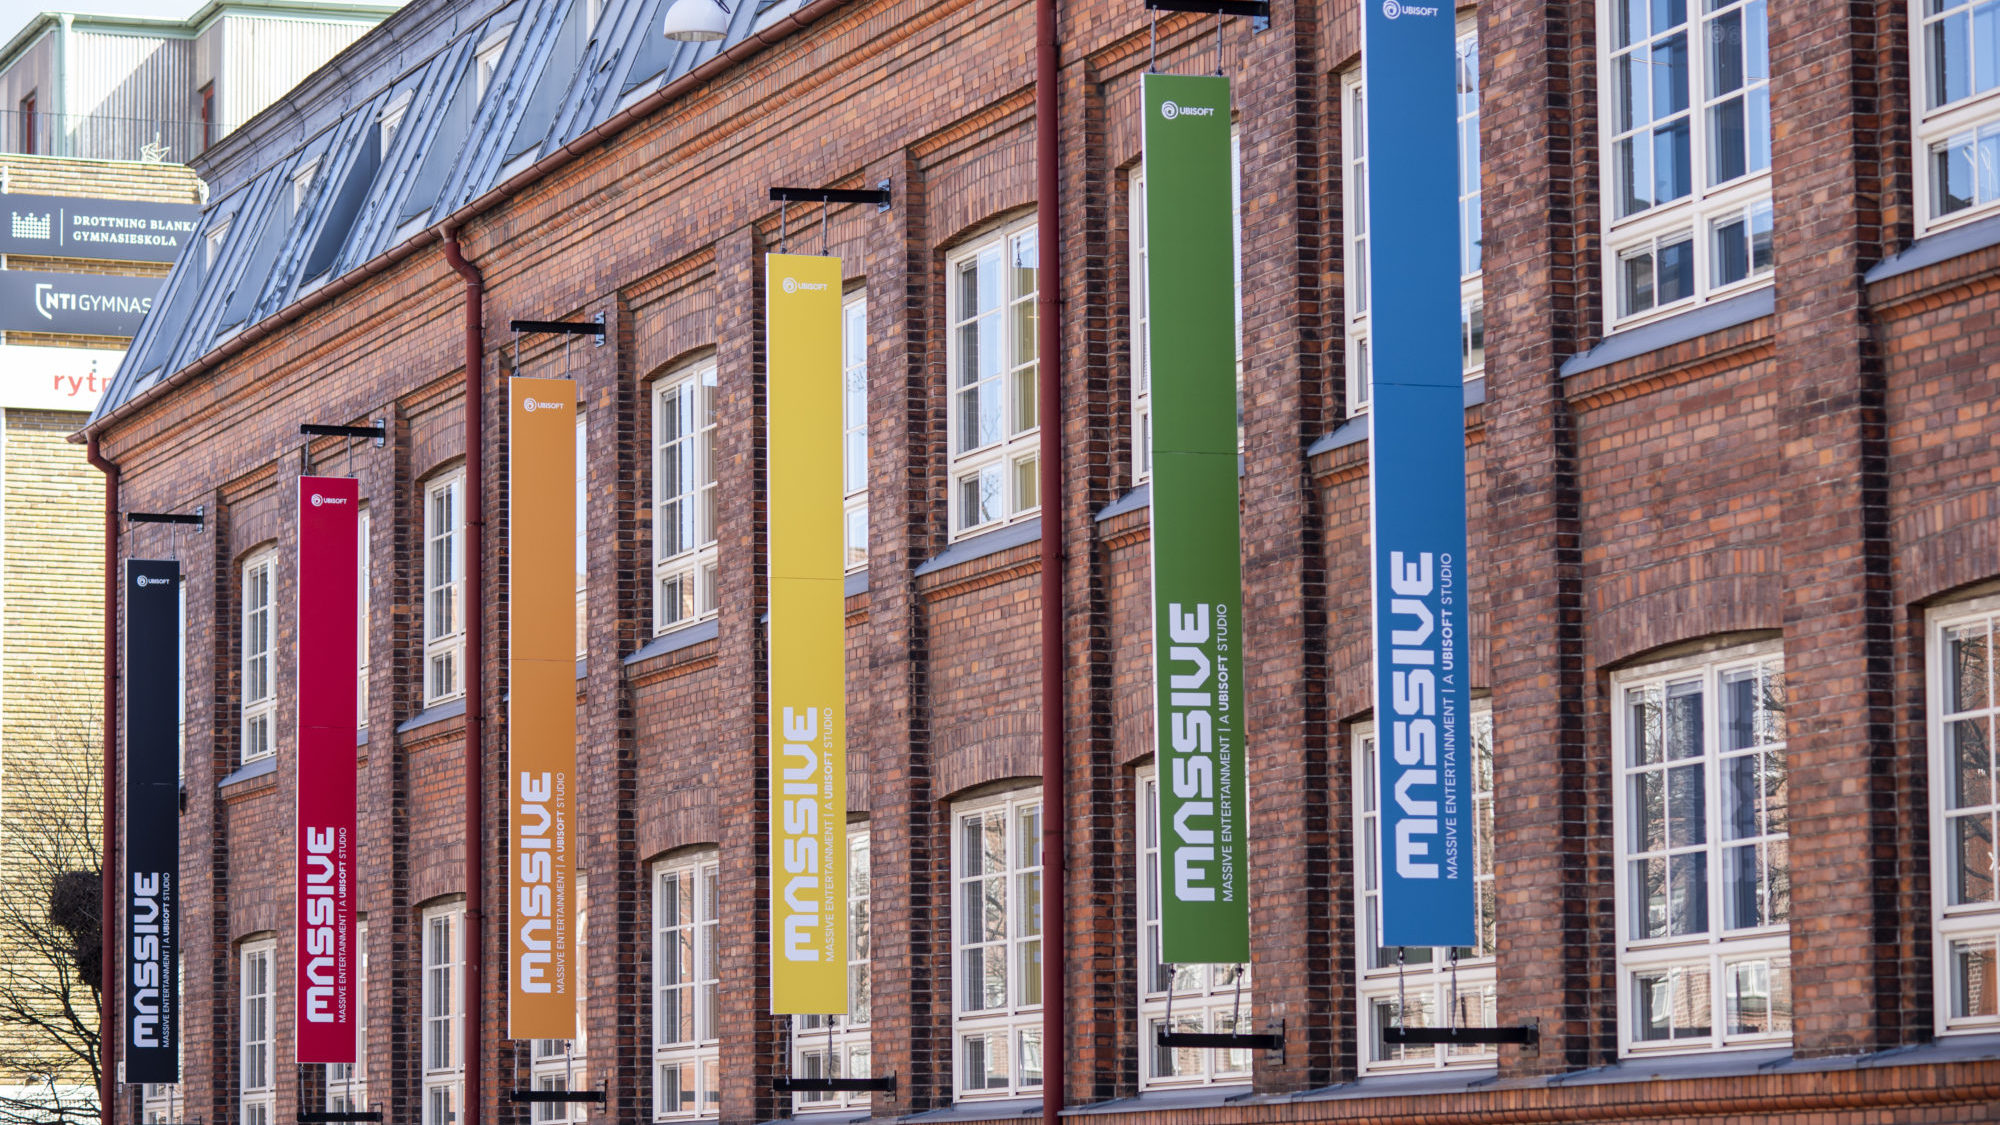
\includegraphics{img/massive_outside.jpg}
  \end{minipage}
\end{frame}

\begin{frame}
  \frametitle{Problem: Communication is good, but hard}
  \begin{minipage}{.49\textwidth}
    \textbf{The science:}
    \begin{shadequote}{}
      the current findings confirm that although sharing information is
      important to team outcomes, teams fail to share information when they
      most need to do so.
    \end{shadequote}
    \vspace{-0.5cm}
    \hspace{0.2cm}
    {\scriptsize-- Information Sharing and Team Performance: A Meta-Analysis} \\
    \ \\
    \textbf{The anecdote:}
    \begin{shadequote}{}
      As soon as we were close the deadline they abandoned <communication-tool>
      and used Post-its instead, because it just works.
    \end{shadequote}
    \vspace{-0.5cm}
    \hspace{0.2cm}
    {\scriptsize-- Manager} \\
  \end{minipage}
  \begin{minipage}{.49\textwidth}
    \hspace{0.5cm}
\includegraphics[width=\textwidth]{img/postits.jpg}
  \end{minipage}
\end{frame}

\begin{frame}
  \frametitle{: Communication is good, but hard}
  \begin{minipage}{.49\textwidth}
    \textbf{The science:}
    \begin{shadequote}{}
      the current findings confirm that although sharing information is
      important to team outcomes, teams fail to share information when they
      most need to do so.
    \end{shadequote}
    \vspace{-0.5cm}
    \hspace{0.2cm}
    {\scriptsize-- Information Sharing and Team Performance: A Meta-Analysis} \\
    \ \\
    \textbf{The anecdote:}
    \begin{shadequote}{}
      As soon as we were close the deadline they abandoned <communication-tool>
      and used Post-its instead, because it just works.
    \end{shadequote}
    \vspace{-0.5cm}
    \hspace{0.2cm}
    {\scriptsize-- Manager} \\
  \end{minipage}
  \begin{minipage}{.49\textwidth}
    \hspace{1.5cm}
\includegraphics[width=0.8\textwidth]{img/error.pdf}
  \end{minipage}
\end{frame}

\begin{frame}
  \begin{center}
    Python Flask
  \end{center}
\end{frame}

\begin{frame}
  \begin{center}
    Development Iteration, User centric.
  \end{center}
\end{frame}

\begin{frame}
  \begin{center}
    Prototype Interfaces.
  \end{center}
\end{frame}

\begin{frame}
  \begin{center}
    Actual Implementation.
  \end{center}
\end{frame}

\begin{frame}
  \begin{center}
    Results.
  \end{center}
\end{frame}

\begin{frame}
  \begin{center}
    Conclusion.
  \end{center}
\end{frame}

\begin{frame}
  \begin{center}
    {\huge
    Thank you for listening! \\
    \vspace{1cm}
    Questions?
    }
  \end{center}
\end{frame}

\end{document}
